\documentclass[10.5pt]{article}
\usepackage{amsmath,amssymb,amsthm}
\usepackage{listings}
\usepackage{graphicx}
\usepackage[shortlabels]{enumitem}
\usepackage{tikz}
\usepackage[margin=1in]{geometry}
\usepackage{fancyhdr}
\usepackage{epsfig} %% for loading postscript figures
\usepackage{amsmath}
\usepackage{float}
\usepackage{amssymb}
\usepackage{caption}
\usepackage{color}
\usepackage{subfigure}
\usepackage{graphics}
\usepackage{titlesec}
\usepackage{mathrsfs}
\usepackage{amsfonts}
\usepackage{indentfirst}
\renewcommand{\baselinestretch}{1.2}%Adjust Line Spacing
%\geometry{left=2.0cm,right=2.0cm,top=2.0cm,bottom=2.0cm}% Adjust Margins of the File
\usepackage{tikz-qtree}
\usetikzlibrary{graphs}
\usetikzlibrary{arrows.meta}
\tikzset{every tree node/.style={minimum width=2em,draw,circle},
	blank/.style={draw=none},
	edge from parent/.style=
	{draw,edge from parent path={(\tikzparentnode) -- (\tikzchildnode)}},
	edge from parent/.append style={<-},
	level distance=30pt,
	sibling distance=5pt}
\setlength{\parindent}{0pt}
%\setlength{\parskip}{5pt plus 1pt}
\setlength{\headheight}{13.6pt}
\newcommand\question[2]{\vspace{.25in}\hrule\textbf{#1: #2}\vspace{.5em}\hrule\vspace{.10in}}
\renewcommand\part[1]{\vspace{.10in}\textbf{(#1)}}
%\newcommand\algorithm{\vspace{.10in}\textbf{Algorithm: }}
\newcommand\correctness{\vspace{.10in}\textbf{Correctness: }}
\newcommand\runtime{\vspace{.10in}\textbf{Running time: }}
\pagestyle{fancyplain}
% Create horizontal rule command with an argument of height
\newcommand{\horrule}[1]{\rule{\linewidth}{#1}}



% Set the title here
\title{
	\normalfont \normalsize
	\textsc{ShanghaiTech University} \\ [25pt]
	\horrule{0.5pt} \\[0.4cm] % Thin top horizontal rule
	\huge CS101 Algorithms and Data Structures\\ % The assignment title
	\LARGE Fall 2021\\
	\LARGE Homework 7\\
	\horrule{2pt} \\[0.5cm] % Thick bottom horizontal rule
}
% wrong usage of \author, never mind
\author{}
\date{Due date: 23:59, October 21, 2021}

% set the header and footer
\pagestyle{fancy}
\lhead{CS101 Algorithms and Data Structures}
\chead{Homework 7}
\rhead{Due date: 23:59, October 21, 2021}
\cfoot{\thepage}
\renewcommand{\headrulewidth}{0.4pt}
\newtheorem{Q}{Question}
% special settings for the first page
\fancypagestyle{firstpage}
{
	\renewcommand{\headrulewidth}{0pt}
	\fancyhf{}
	\fancyfoot[C]{\thepage}
}

% Add the support for auto numbering
% use \problem{title} or \problem[number]{title} to add a new problem
% also \subproblem is supported, just use it like \subsection
\newcounter{ProblemCounter}
\newcounter{oldvalue}
\newcommand{\problem}[2][-1]{
	\setcounter{oldvalue}{\value{secnumdepth}}
	\setcounter{secnumdepth}{0}
	\ifnum#1>-1
	\setcounter{ProblemCounter}{0}
	\else
	\stepcounter{ProblemCounter}
	\fi
	\section{Problem \arabic{ProblemCounter}: #2}
	\setcounter{secnumdepth}{\value{oldvalue}}
}
\newcommand{\subproblem}[1]{
	\setcounter{oldvalue}{\value{section}}
	\setcounter{section}{\value{ProblemCounter}}
	\subsection{#1}
	\setcounter{section}{\value{oldvalue}}
}

% \setmonofont{Consolas}
\definecolor{blve}{rgb}{0.3372549 , 0.61176471, 0.83921569}
\definecolor{gr33n}{rgb}{0.29019608, 0.7372549 , 0.64705882}
\makeatletter
\lst@InstallKeywords k{class}{classstyle}\slshape{classstyle}{}ld
\makeatother
\lstset{language=C++,
	basicstyle=\ttfamily,
	keywordstyle=\color{blve}\ttfamily,
	stringstyle=\color{red}\ttfamily,
	commentstyle=\color{magenta}\ttfamily,
	morecomment=[l][\color{magenta}]{\#},
	classstyle = \bfseries\color{gr33n}, 
	tabsize=4
}
\lstset{basicstyle=\ttfamily}
\begin{document}

\maketitle
\thispagestyle{firstpage}
%\newpage
\vspace{3ex}

\begin{enumerate}
	\item Please write your solutions in English.

	\item Submit your solutions to gradescope.com.

	\item Set your FULL NAME to your Chinese name and your STUDENT ID correctly in Account Settings.

	\item If you want to submit a handwritten version, scan it clearly. Camscanner is recommended.

	\item When submitting, match your solutions to the according problem numbers correctly.

	\item No late submission will be accepted.

	\item Violations to any of the above may result in zero grade.
\end{enumerate}
\newpage

\question{1}{(4$\times1$')Single Choice}


The \textbf{question1-4} are single choice questions, each question has \textbf{only one} correct answer. Select the
correct answer.\\
\textit{Note that you should write you answers of \textbf{question1-4} in the box below.}
\begin{table}[htbp]
	\begin{tabular}{|p{2cm}|p{2cm}|p{2cm}|p{2cm}|}
		\hline
		Question 1 & Question 2 & Question 3 & Question 4 \\
		\hline
		A          & C          & C          & C          \\
		\hline
	\end{tabular}
\end{table}

\begin{Q} A union tree, used in a disjoint set with only union-by-size optimization, has height 6. The number of nodes contained in that tree \textbf{can not} be \_\_\_\_\_.
	\begin{enumerate}[(A)]
		\item 63
		\item 64
		\item 65
		\item 80
	\end{enumerate}
\end{Q}

\begin{Q}Which of the following statements is true?
	\begin{enumerate}[(A)]
		\item If a graph with n vertices has $n-1$ edges, it must be a tree.
		\item A directed graph with n vertices has at least 2n edges to ensure the whole graph is strongly connected.
		\item Both the time complexity of DFS and that of BFS on graph are $\Theta(|V|+|E|)$ .
		\item Every edge is visited exactly once in one iteration of DFS on a connected, undirected graph.
	\end{enumerate}
\end{Q}

\begin{Q}
	Suppose you have an directed graph containing $|V|$ nodes. What is the maximum number of edges you can add to this graph while maintaining it acyclic? (Assume that you are not allowed to add parallel edges.)
	\begin{enumerate}[(A)]
		\item $|V|$
		\item $|V|(|V|+1)/2$
		\item $|V|(|V|-1)/2$
		\item $|V|^2$
	\end{enumerate}
\end{Q}

\begin{Q}Which of the following statements is false?
	\begin{enumerate}[(A)]
		\item In a directed simple graph, the maximal number of edges is $|V|(|V|-1)$.
		\item Undirected graph $G = (V, E)$ is stored in an adjacency matrix $A$. The degree of $V_i$ is $\sum_{j=1}^{|V|}A[i][j]$.
		\item A DFS of a directed graph always produces the same number of tree edges, i.e.
		      independent of the order in which the vertices are considered for DFS.
		\item In BFS, let $d(v)$ be the minimum number of edges between a vertex $v$ and the start vertex. For any two vertices $u, v$ in the fringe, $|d(u)-d(v)|$ is always less than 2.

	\end{enumerate}
\end{Q}

\pagebreak
%%%%%%%%%%%%%%%%%%%%%%%%%%%%%
\question{2}{(2$\times$2') Disjoint set practice}
Given the following set of operations on a disjoint set,
show the final disjoint set tree for each of the following optimization strategies.\\
$set\_union(A, D),\ set\_union(C, B),\ set\_union(F, E),\ set\_union (G, C),$\\
$set\_union(D,G),\ find(A),\ set\_union(H, E),\ set\_union(E,G),\ find(E)$\\
\\
(1)(2') Only with union-by-size optimization. (When two trees have the same height, the set specified first in the union will be the root of the merged set.)\\
\begin{center}
	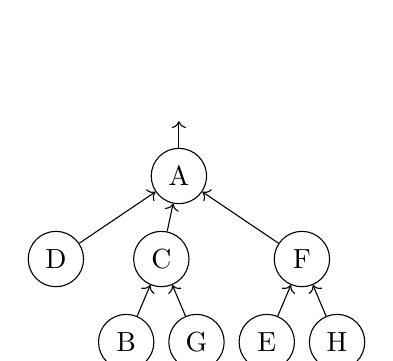
\begin{tikzpicture}
		\Tree
		[.\node[blank]{};
		[.A D
			[.C B G
			]
			[.F E H
			]
		]
		]
	\end{tikzpicture}
\end{center}
(2)(2') Only with path compression. (The set specified first in the union will always be
the root of the merged set.)\\
\begin{center}
	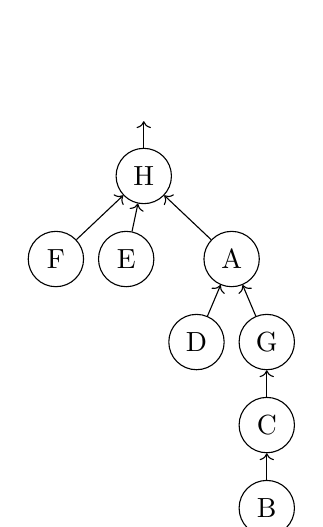
\begin{tikzpicture}
		\Tree
		[.\node[blank]{};
		[.H F E
			[.A D
					[.G
							[.C B
							]
					]
			]
		]
		]
	\end{tikzpicture}
\end{center}
\pagebreak
%%%%%%%%%%%%%%%%%%%%%%%%%%%%%

\question{3}{(3$\times$2') Graph traversal practice}

\begin{figure}[htbp]
	\centering
	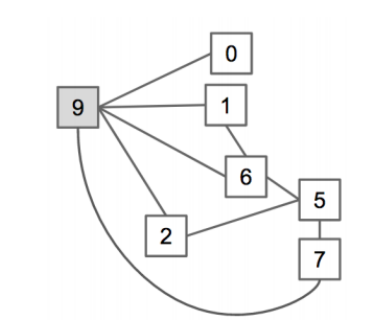
\includegraphics{graph_traversal.png}
	\label{fig:my_label}
\end{figure}
\begin{itemize}
	\item[(a)] For the graph above, give the depth first search preorder traversal starting from vertex 9, assuming that we break ties by visiting smaller numbers first.\\
	      9, 0, 1, 6, 5 ,2 7
	\item[(b)] For the graph above, give the depth first search postorder traversal starting from vertex 9, assuming that we break ties by visiting smaller numbers first.\\
	      0, 2, 7, 5, 6, 1, 9
	\item[(c)] For the graph above, give the breadth first search traversal starting from vertex 9, assuming that we break ties by visiting smaller numbers first.\\
	      9, 0, 1, 2, 6, 7, 5
\end{itemize}

\pagebreak
%%%%%%%%%%%%%%%%%%%%%%%%%%%%%
\question{4}{(4') DFS went wrong!}
The following algorithm which runs DFS on a directed graph, but it contains an fatal error.
\begin{lstlisting}
    Create a stack.
    Choose the initial vertex and mark it as visited.
    Put the initial vertex onto the stack.
    while the stack is not empty:
        Pop a vertex V from the top of the stack.
        for each neighbor of V:
            if that neighbor is not marked as visited:
                Mark that neighbor as visited.
                Push that neighbor onto the stack.
\end{lstlisting}

Please give a graph as an counterexample and briefly explain why this algorithm is wrong.
\\
\textit{Note: In this problem, we say a node is "visited" whenever it is marked as visited.}\\
\begin{center}
	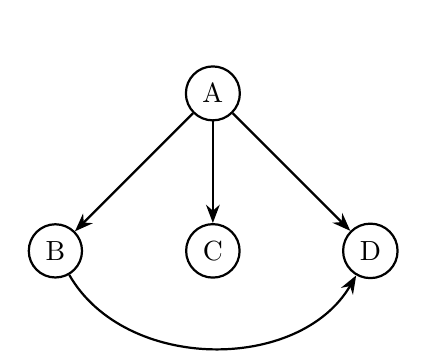
\begin{tikzpicture}
		\begin{scope}[every node/.style={circle, thick, draw}]
			\node(A) at (0, 0) {A};
			\node(B) at (-2, -2){B};
			\node(C) at (0, -2) {C};
			\node(D) at (2, -2) {D};
		\end{scope}
		\begin{scope}[>={Stealth[black]}, every edge/.style={draw=black,thick}]
			\path [->] (A) edge (B);
			\path [->] (A) edge (C);
			\path [->] (A) edge (D);
			\path [->] (B) edge[bend right=60] (D);
		\end{scope}
	\end{tikzpicture}
\end{center}
In the above graph, the correct DFS order (preorder) from node $A$ should be $A, B, D, C$, or $A, C, B, D$, or $A, C, D, B$, or $A, D, B, C$, or $A, D, C, B$. However, the algorithm above will give $A, B, C, D$,or $A, B, D, C$ or $A, C, B, D$, or $A, C, D, B$, or $A, D, B, C$, or $A, D, C, B$. The order $A, B, C, D$ is wrong.This is because $D$ is marked as visited while it actually haven't been visited. The problem of the algorithm is that the vertex should be marked as visited when poped, not pushed. It can be modified as follows.
\begin{lstlisting}
	Create a stack.
	Choose the initial vertex and mark it as visited.
	Put the initial vertex onto the stack.
	while the stack is not empty:
			Pop a vertex V from the top of the stack.
			if V is not marked as visited:
					Mark V as visited.
			for each neighbor of V:
					if that neighbor is not marked as visited:
							Push that neighbor onto the stack.
\end{lstlisting}

\pagebreak
%%%%%%%%%%%%%%%%%%%%%%%%%%%%%
\question{5}{(2'+3') Bipartite graph}

A bipartite graph, $G = (V,E)$, is a graph such that V can be partitioned into two subsets $V_1$ and $V_2$
and no edge has both its vertices in the same subset. See the figure below.

\begin{figure}[htbp]
	\centering
	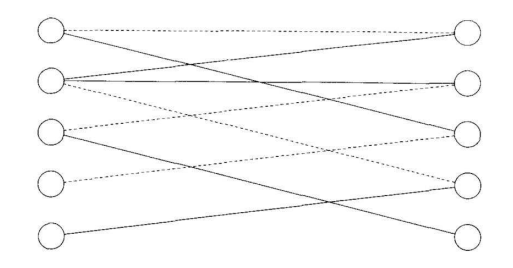
\includegraphics{bipartite_graph.png}
	\label{fig:my_label}
\end{figure}

(a) Show that every tree is a bipartite graph.\\
\\
Firstly, put root into $V_1$. For each node in the tree, if its parent is in $V_1$, put the node into $V_2$, else put the node into $V_1$. Since each node are connected noly to its parent and children, the previous construction method, each node are in the different set to its parent and children, it doesn't connect to any other node in the same set. Therefore, each tree is a bipartite graph.\\
\\
(b) The bipartite matching problem is to find the largest subset $E'$ of $E$ such that no vertex is
included in more than one edge. A matching of four edges (indicated by dashed edges) as
\\
Suppose now you have the solution of bipartite matching problem, let's call it algorithm $A$. Show how the bipartite matching problem can be used to solve the following problem: We have
a set of workers, a set of tasks, and a list of tasks that each worker is qualified to finish.
If no worker is required to finish more than one task, and each worker can only finish his qualified tasks, what is the maximum number of tasks that can be finished?\\
(You just need to show how to construct this problem as one bipartite matching problem, and do not need to give the detail of algorithm $A$.)\\
\\
We see both workers and tasks as vertices in the graph. If a worker is qualified to finish the task according to the list, the worker vertex and the task vertex are connected. Since no connection among workers, nor among tasks, the graph is a bipartite graph $G(V, E)$ with worker vertices been put into $V_1$ and task vertices been put into $V_2$. The degree of the worker vertices indicates the number of tasks the worker is going to finish and the degree of the task vertex indicates the how many times it is to be finished. No worker is required to finish more than one task, and no task need to be finished more than once (of course). Therefore, no vertex is included in more than one edge.(*) We want to find the maximum number of tasks that can be finished means we want to find the largest subsets of $E$ meets the previous constraint (*). This is a bipartite matching problem.\\
\pagebreak

\end{document}